\chapter{ScatterPlot View}
\label{sec:scatter_view}

A ScatterPlot View displays the distribution of two numerical variables as points. When started, it presents itself in the following manner.

\begin{figure}[H]
    \hspace*{-2cm}
    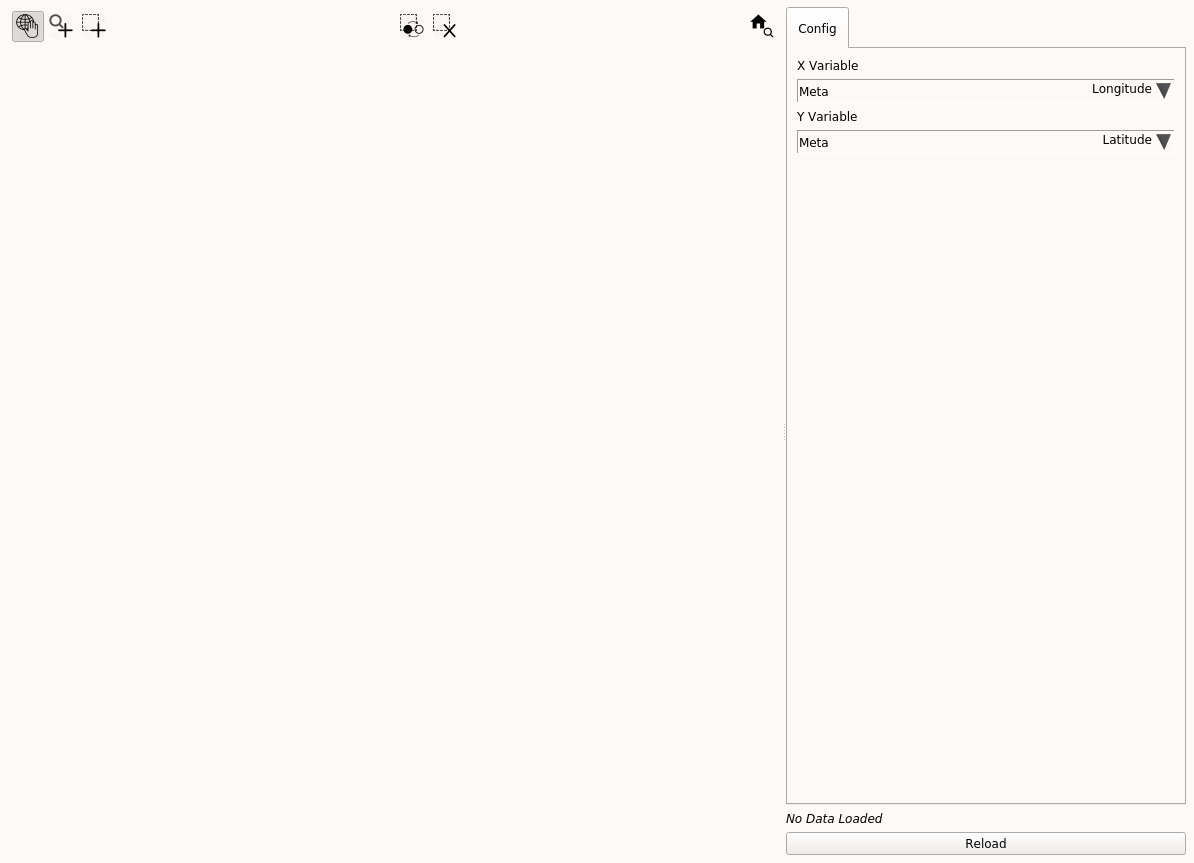
\includegraphics[width=18cm,frame]{figures/scatter_start.png}
  \caption{Scatterplot View startup}
\end{figure}

\section{Layout}

At the top, a  tool bar is shown, showing the currently selected tool and the available actions. \\

On the left side, the data is shown (if data has been loaded). \\

On the right side, a configuration area exists which allows configuration of what data is loaded and how it is displayed. \\

Both areas can be resized and hidden if wanted.

\section{Data Loading}

To load the data the mechanism described in Section \nameref{sec:load} or the 'Reload' button can be used. To filter the dataset, the mechanism described in Section \nameref{sec:filtering} can be used. \\

\begin{figure}[H]
    \hspace*{-2cm}
    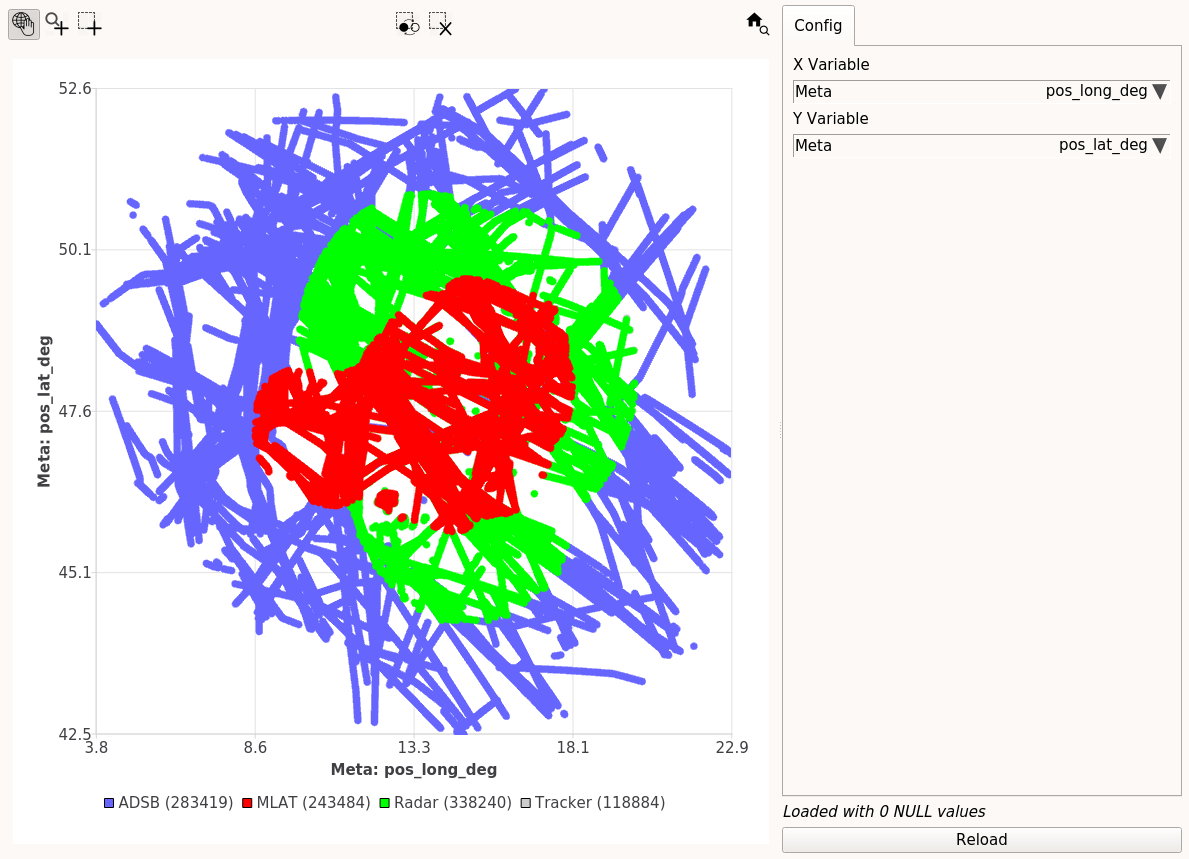
\includegraphics[width=18cm,frame]{figures/scatter_loaded.png}
  \caption{Scatterplot View after loading}
\end{figure}

The value of selected variables is used for positioning on x-axis and y-axis, the color is defined by DBObject. On the bottom a legend is shown giving the total counts of all data points. \\

In the current example the meta-variables 'tod' is used, showing the overall data rate per DBObject.

On the bottom a legend is shown giving the total counts of all data points. \\

In the current example the WGS-84 meta-variables 'pos\_long\_deg' and 'pos\_lat\_deg' are used, showing a similiar view as OSGView.


\section{Usage}

\subsection{Toolbar}

The first symbols switch between the mouse action modes:

\begin{table}[H]
  \center
  \begin{tabular}{ | l | l | l |}
    \hline
    \textbf{Icon} & \textbf{Text} &  \textbf{Description} \\ \hline
    \includegraphics[width=0.5cm,frame]{../../data/icons/navigate.png} & Navigate & Allows navigation of the data \\ \hline
    
\includegraphics[width=0.5cm,frame]{../../data/icons/zoom_select_action.png} & Zoom to Rectangle & Allows zooming to the selected rectangle \\ \hline
    
\includegraphics[width=0.5cm,frame]{../../data/icons/select_action.png} & Select & Allows data selection \& de-selection \\ \hline
  \end{tabular}
  \caption{Toolbar mouse action modes}
\end{table}

The others provide general operations (shortcut refers to keyboard shortcut):

\begin{table}[H]
  \center
  \begin{tabular}{ | l | l | l | l |}
    \hline
    \textbf{Icon} & \textbf{Shortcut} &\textbf{Text} &  \textbf{Description} \\ \hline
    \includegraphics[width=0.5cm,frame]{../../data/icons/select_invert.png} & & Invert Selection & Selects all de-selected \& vice versa \\ \hline
    \includegraphics[width=0.5cm,frame]{../../data/icons/select_delete.png} & & Delete Selection & De-selects all target reports \\ \hline
    \includegraphics[width=0.5cm,frame]{../../data/icons/zoom_home.png} & & Zoom to Home & Pans/zooms to show all existing data \\ \hline
  \end{tabular}
  \caption{Toolbar operations}
\end{table} 

\subsection{Config Tab}

The top elements define which data variables are used for the x/y-axis, which can be any numerica) variable (might require a reload operation). \\

Please note that display of evaluation result data is currently not implemented. \\

The 'Reload' button can be used to trigger a reload.

\subsection{Scatterplot}

\subsubsection{Zoom}

The mouse wheel can be used to zoom in or out of the presented data, the space key can be used to reset to the default zoom (euqivalent to \includegraphics[width=0.5cm,frame]{../../data/icons/zoom_home.png}).

\subsubsection{Navigate Action}

In the 'Navigate mode', the left mouse-button can be used to pan the viewabled data.

\subsubsection{Zoom to Rectangle Action}

In the 'Zoom to Rectangle' mode, the left mouse-button can be used to select a rectangle, to which a zoom operation is performed.

\subsubsection{Select Action}

Using the default action data can be selected. The first left mouse-button click starts selection (showing a red rectangle), the second click finalizes the selection. All data in all intersected bins is selected.

\begin{figure}[H]
    \hspace*{-2cm}
    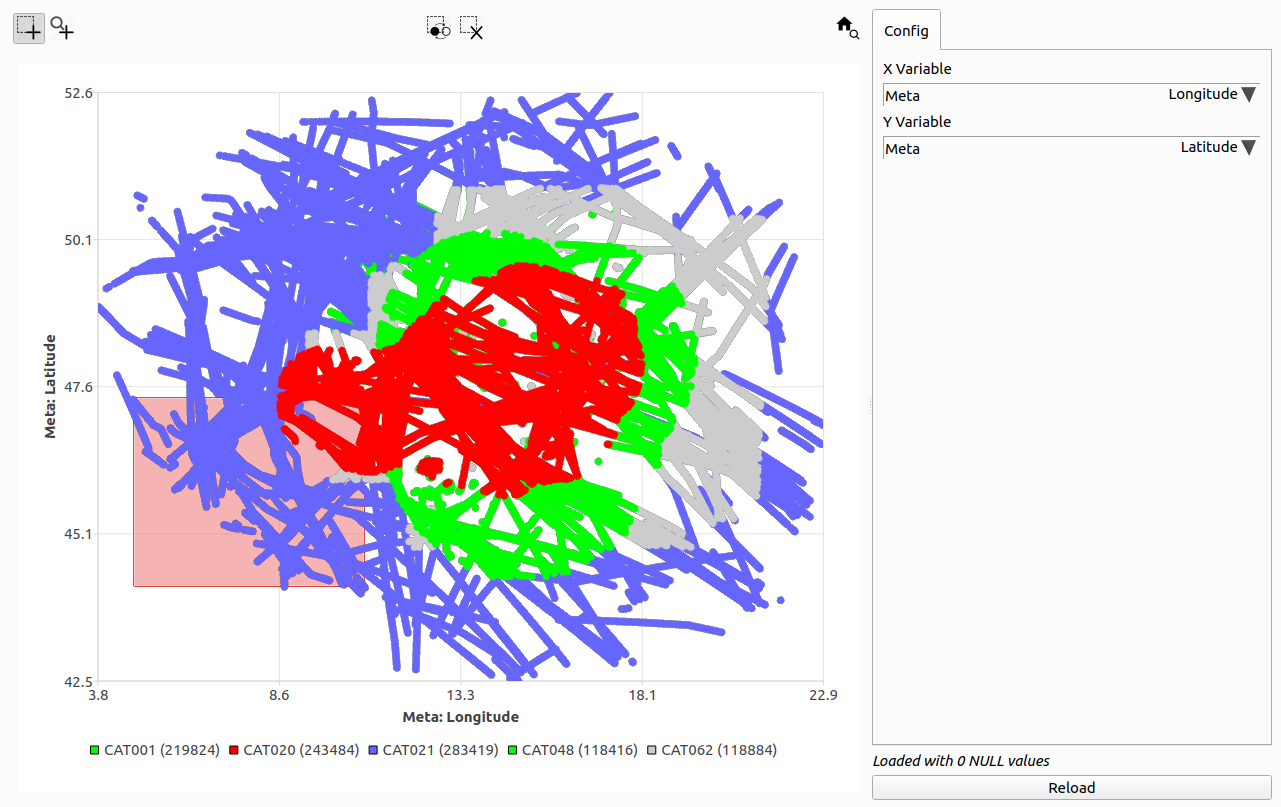
\includegraphics[width=18cm,frame]{figures/scatter_select.png}
  \caption{Scatterplot View data selection}
\end{figure}

The selected data is then presented in an extra 'Selected' column, grouping the count of all DBOObjects.

\begin{figure}[H]
    \hspace*{-2cm}
    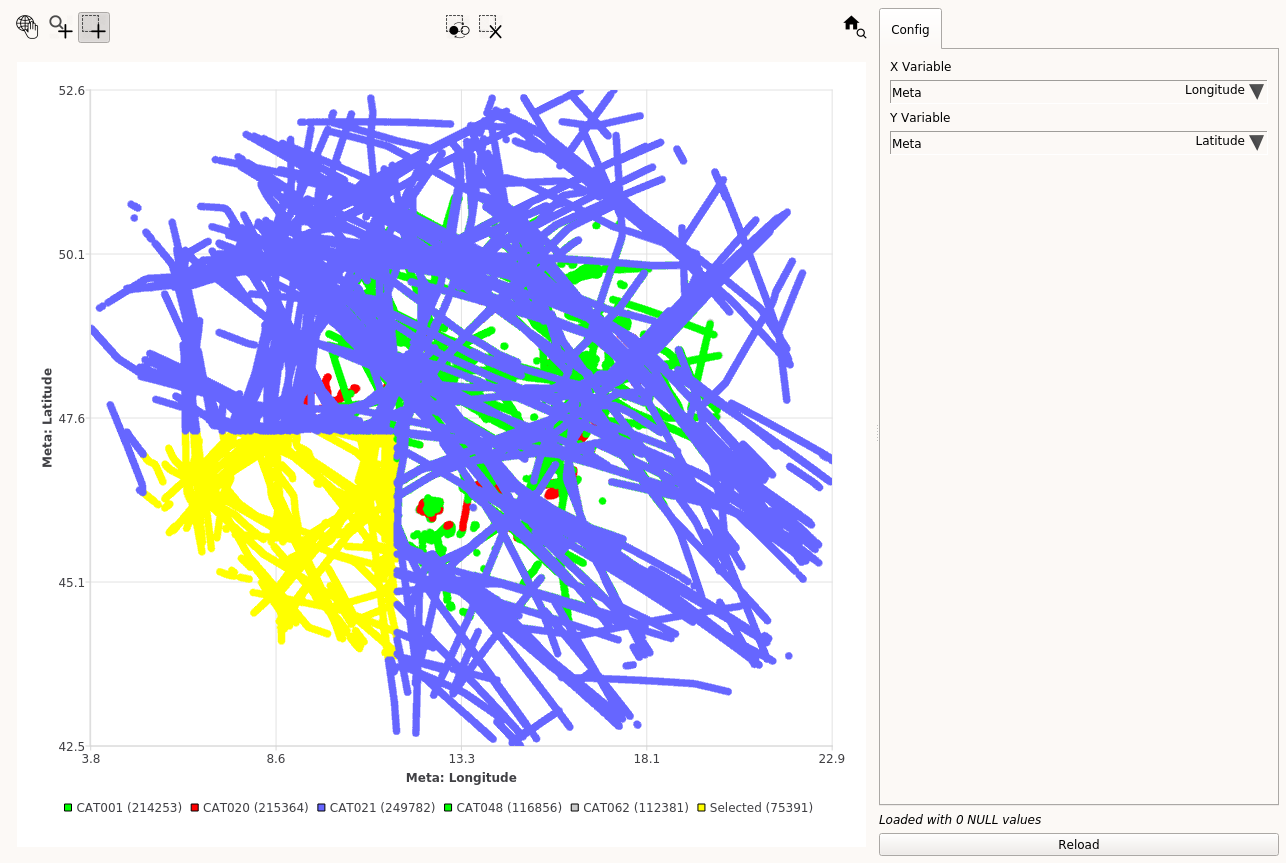
\includegraphics[width=18cm,frame]{figures/scatter_selected.png}
  \caption{Scatterplot View data selected}
\end{figure}

This allows selection of parts of the data based on the presented variable, allowing deeper analysis e.g. of dubious data. \\

The 'Invert Selection' \includegraphics[width=0.5cm,frame]{../../data/icons/select_invert.png} or 'Delete Selection' \includegraphics[width=0.5cm,frame]{../../data/icons/select_delete.png} actions allow for easier selection of the wanted target reports. \\

Also, if the 'Control' key is pressed during the second click, the new selected data is added to the already existing collection.









